\documentclass{article}

%% The amssymb package provides various useful mathematical symbols

\usepackage{amssymb}
\usepackage{microtype}
\usepackage{subfigure}
\usepackage{booktabs} % for professional tables
\usepackage{xr}
\usepackage{times}
\usepackage{float} % for figure placement
\usepackage{amsmath}
\usepackage{graphicx}

 

% hyperref makes hyperlinks in the resulting PDF.

% If your build breaks (sometimes temporarily if a hyperlink spans a page)

% please comment out the following usepackage line and replace

% \usepackage{icml2021} with \usepackage[nohyperref]{icml2021} above.

\usepackage{hyperref}

% Attempt to make hyperref and algorithmic work together better:

\newcommand{\theHalgorithm}{\arabic{algorithm}}

% Use the following line for the initial blind version submitted for review:

\usepackage{icml2023}

 

\icmltitlerunning{On the Estimation of Gaussian Mixture Copula Models}

 

\begin{document}

\twocolumn[

\icmltitle{On the Estimation of Gaussian Mixture Copula Models}

 

\icmlsetsymbol{equal}{*}

 

\begin{icmlauthorlist}

\icmlauthor{Aeiau Zzzz}{equal,to}

\end{icmlauthorlist}

 

\icmlaffiliation{to}{Department of Computation, University of Torontoland, Torontoland, Canada}

\icmlcorrespondingauthor{Ashutosh Tewari}{ashutosh80@gmail.com}

 

% You may provide any keywords that you

% find helpful for describing your paper; these are used to populate

% the "keywords" metadata in the PDF but will not be shown in the document

\icmlkeywords{Copulas, Density estimation, Normalizing flows, Mixture models}

 

\vskip 0.3in

]

 

\DeclareRobustCommand{\nativellDenom}[1] {\prod\limits_{r=1}^{d}\psi_{r}\left(\Psi^{-1}_{r} \left( \bs{u}_r{#1} \right);\Theta^r \right) }

\DeclareRobustCommand{\llDenom}[1] {\prod\limits_{r=1}^{d}\psi_{r}\left(Z_{r{#1}};\Theta^r \right) }

\DeclareRobustCommand{\invCDF}[1]{ Z_{#1} }

\DeclareRobustCommand{\erf}{\textmd{erf}}

\DeclareRobustCommand{\AltllDenom}[1] {\log \left( \psi_{r}\left(\Psi^{-1}_{r} \left( \bs{u}_{r#1} \right);\Theta^r \right) \right) }

\DeclareRobustCommand{\zbar}[1] {\bar{Z}_{:{#1}}}

\DeclareRobustCommand{\ma_zbar}[2] {\bar{\textbf{z}}_{#1}(#2)}

\DeclareRobustCommand{\der}[2] {\frac{\partial \left({#2}\right)}{\partial {#1}}}

\newcommand{\bs}[1]{\boldsymbol{#1}}

\DeclareRobustCommand{\bf}[1]{\textbf{#1}}

\newcommand{\argmaxI}{\mathop{\mathrm{argmax}}\nolimits} % ASdeL

 

 

 

%\printAffiliationsAndNotice{}  % leave blank if no need to mention equal contribution

\printAffiliationsAndNotice{\icmlEqualContribution} % otherwise use the standard text.

 

\begin{abstract}

This paper revisits Gaussian Mixture Copula Model (GMCM), a more expressive alternative to the widely used Gaussian Mixture Model (GMM), to make its parameter estimation tractable. Both the Expectation Maximization and the direct Likelihood Maximization frameworks for GMCM have to grapple with a likelihood function that lacks a closed-form. This has led to a few approximation schemes that alleviate the problem, nonetheless leaving the issue still unresolved.  Additionally, past works have alluded to an additional challenge of parameter unidentifiability, but none has offered a rigorous treatment and a commensurate solution framework to overcome the same. This work offers solutions to each of these issues in an attempt to help GMCM realize its full potential. The source of unidentifiability is not only proven but also suitable priors are proposed that eliminate the problem. Additionally, an efficient numerical framework is proposed to evaluate the intractable likelihood function, while also providing its analytical derivatives. Finally, a view of GMCM as a series of bijective mappings from a base distribution is presented, which paves the way to synthesize GMCM using modern, probabilistic programming languages (PPLs). The main claims of this work are supported by empirical evidence gathered on synthetic and real-world data sets.

 

% a likelihood function that lacks a closed-form representation, and the reliance on numerical gradients (of likelihood function) make the parameter estimation cost prohibitive and impractical for high-dimensional, high-volume data-sets.

 

 

% for modeling continuous, multivariate data-sets, exhibiting multimodal distribution. GMCM combines the complex dependencies  endowed to Like other copula-based models, the strength of GMCMs comes from the ability to separate the learning of marginal models of the random variables from that of the dependence between them. Despite this flexibility and its potential impact on modeling real-world data, the learning of GMCM parameters is hard. The issue of non-identifiability, an intractable likelihood function that lacks a closed-form representation, and the reliance of maximum-likelihood methods on numerical gradients make the parameter estimation cost prohibitive and impractical for high-dimensional problems. This work offers solutions to each of these issues in an attempt to help GMCM realize its full potential. The main claims of this work are supported with empirical evidences shown on simulated and real-world data-sets.

\end{abstract}

 

%% \linenumbers

 

%% main text

\section{Introduction}\label{sec:Intro}

Modeling multivariate data is of fundamental interest in several domains to solve myriad of practical problems. From a probabilistic viewpoint, it amounts to defining a generative process that best explains the observed data when seen as random variables. Copulas provide a unique framework to model multivariate data that allows for a complete control on the marginal behaviors of the random variables, while being able to separately capture the dependencies between them. See \citep{Durante2010CopulaIntro} and references therein for a succinct monograph on this subject with a brief historical perspective.  The decoupling $-$of marginal and joint behavior$-$ induced by a copula can be especially significant when the true data generating process imposes strict constraints over the marginal distributions of some/all random variables. Ideally, any effort to model such data should adhere to these constraints. However, in the pursuit of finding a joint model of the random variables, one typically ends up with inconsistent marginal models.  Given the ability of copulas to overcome such inconsistencies, they have been applied in many scientific fields though particularly in finance \citep{Genest2009CopulaInFinance,Cherubini2004copula}, reliability analysis \citep{Rychlik2010Reliability} and molecular biology \citep{Bilgrau2012quantification,Li2011,Kim2008,Ma2012Gini}.  There has also been  attempts to find synergies between copula theory and machine learning to build high fidelity data-driven models \citep[see][for a survey on the applications of copulas in machine learning approaches]{Elidan2013}.

The focus of this paper is on multivariate problems with continuous random variables, exhibiting multimodal behavior in their  joint (and/or marginal) distribution. Gaussian Mixture Models (GMMs) \citep{Bilmes98agentle} have been prolifically used to model such data-sets, thanks to their simplicity and an efficient Expectation-Maximization (EM) algorithm for parameter estimation. However, the assumption of jointly normally distributed components is frequently violated in real-world applications, with unintended practical ramifications. Gaussian mixture copula model (GMCM) \citep{Tewari2011,Bilgrau2016,Bhattacharya2014} offers a more expressive alternative to GMM, as illustrated in Figure \ref{fig:motivating_example_gmcm}. A synthetic two-dimensional dataset with 100 samples (Figure \ref{fig:motivating_example_gmcm}a) appears to have a bimodal distribution with non-Gaussian modes. The best-fit GMCM and a GMM are obtained on this dataset, wherein the optimal number of components is determined via the widely used Bayesian Information Criterion (BIC). A quick look at the density contours (Figure \ref{fig:motivating_example_gmcm}b-\ref{fig:motivating_example_gmcm}c) and the generated random samples (Figure \ref{fig:motivating_example_gmcm}d-\ref{fig:motivating_example_gmcm}e), suggests that the GMCM is a more faithful model of the underlying data, with a noticeable tighter fit. The GMM, on the other hand, can be seen to diffuse into regions with no data support, even with an extra mixing component.

\begin{figure}[ht]
\centering
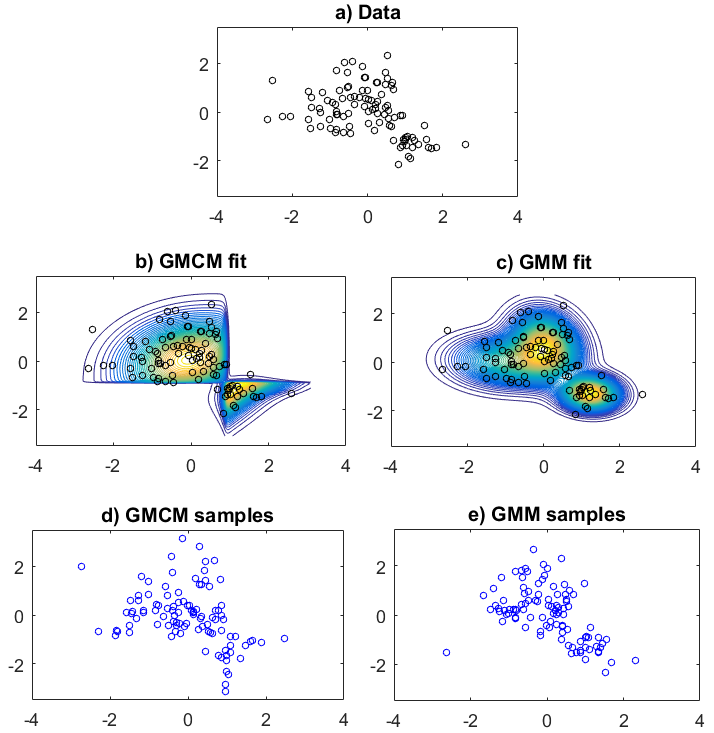
\includegraphics[width= 240pt,height=275pt]{figures/figure_for_motivating_gmcm}
\caption{(a) A 2-dimensional dataset with 100 samples, (b-c) contours of best-fit GMCM (with 2 components) and GMM (with 3 components), (d-e) 100 random samples generated from the two fitted distributions. A tighter fit and a closer resemblance of the random samples to that of training dataset, suggest the GMCM to be a superior generative model of the data than the GMM.}
\label{fig:motivating_example_gmcm}
\end{figure}

Despite its superior expressivity, the estimation of GMCM parameters remains a challenge primarily due to three reasons that we briefly mention here and later explain. First, GMCMs suffer from an inherent issue of \emph{parameter unidentifiability}. Second, its likelihood function does not admit a closed analytical form, and thus not amenable to the EM framework for parameter estimation. Third, concomitant of the second reason, even the direct likelihood maximization (via gradient-based methods) becomes hard due to the lack of analytical gradients (numerical gradients are computationally expensive). The main contributions of this paper address each of these issues i.e. 1) additional conditions are specified that provably mitigate the unidentifiability of GMCM, 2) a correct formulation of EM algorithm for GMCM is presented, 3) a numerical scheme is proposed to approximate GMCM's likelihood function, while providing analytical gradient for the same, and 4) a view of GMCM as a series of bijective mappings is presented that makes it amenable to modern probabilistic programming frameworks and leverage their built-in automatic differentiation capabilities.

The plan of this paper is as follows. Sections \ref{subsec:LitReview} and \ref{subsec:Notation} present a short literature review on this topic, and set the notations to be used in rest of the paper, respectively. Section \ref{sec:GMC_description} describes the GMCM framework and highlights the challenges with the estimation of its parameters. The source of unidentifiability of GMCM is discussed in section \ref{sec:identifiability_GMCM} and a solution is proposed. Section \ref{sec:BijMap} presents a view of GMCM as a series of bijective mappings over a mixture of Gaussians as the base distribution.   \ref{sec:NumLike}, a numerical scheme is proposed to evaluate the likelihood function, while   

an EM algorithm for GMCM, which becomes nontrivial owing to its intractable likelihood function. Section \ref{sec:Derivatives} derives analytical gradient needed to perform the M-step of the EM algorithm. Results on synthetic datasets are included in section \ref{sec:Experimental} to corroborate the claims, before concluding in section \ref{sec:Conclusion&FutureWork} with remarks on a few future research directions.

\subsection{Related work on construction of multivariate Copulas}\label{subsec:LitReview}

The literature on copulas has been dominated by bivariate copula models with a rich set of parametric families to choose from \citep{Nelsen1999introduction}. Although the idea of higher dimensional copula construction is not new \citep[see][]{Genest1995Multivariate, Joe1993Multivariate,Kojadinovic2010RpackageMVcopula}, the literature on it is relatively recent. For instance, \citet{Bedford2002,Kurowicka2009Book,Czado2010PairCopula} proposed  synthesis of multivariate copula from bivariate copulas by assuming a tree-structured dependency between the random variables. This idea was extended to directed acyclic graphs \citep[see][]{Elidan2010,Hanea2006CBN},  giving rise to \emph{Copula Bayesian Networks}. In high-dimensional settings, the recovery of sparse inverse covariance structure of a Gaussian copula was studied by \citet{Liu2009} yielding  \emph{non-paranormal} models.

Copula-based construction to address multi-modality \textemdash \ a frequently observed trait in real-world data\textemdash was first addressed by \citet{Tewari2011} with the proposal of GMCM. \citet{Bilgrau2016} furthered this work by noting certain challenges with the parameter estimation of GMCM and proposed practical solutions for the same. This was coupled with an improved implementation of the model as an open-source package \citep{Bilgrau_Rpackage} in R. \citet{Rajan2016_GMCM_mixed_data} extended GMCM to construct flexible generative models for mixed (continuous and discrete) data-types. The role of automatic differentiation, to obtain gradients of GMCM's intractable likelihood function, was explored by \citet{kasa2018}. Nevertheless, none of these works rigorously addressed the issues stemming from parameter unidentifiability of GMCM and the intractability of its likelihood function (and its gradient), thereby providing the motivation for this work.

Recently, there have been some interesting developments in the area of \emph{model-based clustering} using copulas \citep{Kosmidis2016,Mazo2017,Marbac2017,Rey2012_CopulaMixture}. The motivation there, is to overcome the restrictive normality assumption by cleverly using copulas, from \emph{known} parametric families, to capture the dependence in each mixing component; for instance the \emph{Gaussian Copula Mixture Model} (GCMM) \citep{Marbac2017} employs Gaussian copula for the same. Although with a very similar motivations (and names), the two lines of work (GMCM and GCMM) are fundamentally different, as the goal in GMCM is to seek a \emph{single} copula distribution to capture the entire multimodal dependence structure. 

Another related (albeit rather remotely) line of work pertains to deep generative models a.k.a \emph{normalizing flows} (NFs), which has garnered significant attention in  the Machine Learning community [REF]. The idea behind these models is to transform a simple base distribution, such as an isotropic Gaussian, via bijective mappings that are carefully crafted using deep neural networks. Endowed with such mappings, one can compose highly expressive generative model for continuous data, resulting in best in class performance for the task of multivariate density estimation. The similarities and dissimilarities are drawn between GMCM and the NF-based models.   

\subsection{Notation}\label{subsec:Notation}
The lowercase letters are used for scalars, lowercase boldface letters for vectors, uppercase letters for matrices and Greek letters for model parameters or functions. Unless otherwise stated, vectors are column vectors. The subscripts are used to denote an element of a vector or a matrix. For example, $\bs{x}_i$ and $X_{ij}$ denote the $i^{th}$ and the $(i,j)^{th}$ elements of a vector $\bs{x}$ and a matrix $X$, respectively. Likewise, $X_{i:}$ (or $X_{:i}$) represents the $i^{th}$ row (or column) of a matrix $X$. The subscripts are also used to indicate dimension-specific functions. For instance, the marginal distribution, induced by a joint distribution $\Psi$, along the $j^{th}$ dimension is denoted as $\Psi_j$.  The superscripts are reserved to indicate parameter association. For example, $\Theta^i$ denotes parameters associated with some entity $i$. Table \ref{tab:symbol_glossary} in appendix \ref{apd:symbol_glossary} lists frequently appearing symbols in the paper for a quick reference.

\section{Gaussian Mixture Copula Model}\label{sec:GMC_description}
\textbf{Definition 1:}  A \emph{m}-component \emph{Gaussian Mixture Copula} (GMC) distribution, parameterized by $\Theta = \{\bs{\mu}^l, \Sigma^l, \alpha^l\}_{l=1}^m$, defines a joint distribution of a vector $\bs{u}$, whose constituent elements are uniformly distributed, i.e. $ \bs{u}_j \sim \text{Uniform(0,1)}, \  j\in \{1,2,\cdots d\}$. The GMC density function given by Equation \eqref{eq:GMC_density}.

\begin{align}\label{eq:GMC_density}
\zeta(\bs{u};\Theta) & = \left( \frac{\psi\left(\Psi^{-1}(\bs{u});\Theta\right)}{\nativellDenom{}} \right)
\end{align}

The symbol $\psi(\cdot;\Theta)$ denotes the joint density function of a GMM parameterized with $\Theta = \{\bs{\mu}^l, \Sigma^l, \alpha^l\}_{l=1}^m$, where $\bs{\mu}^l \in \mathbb{R}^d$, $\Sigma^l \in \mathbb{S}_+^d$ and $\alpha^l \in \mathbb{R}^+ \text{s.t.} \sum \alpha^l=1$ denote the mean vector, the covariance matrix and the mixing proportion of the $l^{th}$ component, respectively. The marginal densities induced by the GMM are denoted by $\psi_r(\cdot;\Theta^r)$, with $\Theta^r\subset \Theta$ being the subset of parameters corresponding to the $r^{th}$ dimension. Also, $\Psi_r(\cdot)$ $\left(\text{and} \ \Psi^{-1}_r(\cdot) \right)$ is the cumulative distribution function (and its inverse) of the GMM along the $r^{th}$ margin, and $\Psi^{-1}(\bs{u})=[\Psi^{-1}_1(\bs{u}_1), \cdots, \Psi^{-1}_d(\bs{u}_d)]$. This definition directly follows from the \emph{inversion method} of constructing copulas from any multivariate distribution (in this case, a Gaussian Mixture distribution) with continuous margins ~\citep[see][chapter 3]{Nelsen1999Chapter3}. Since all the elements of a sample $\bs{u}\in [0,1]^d$ from GMC distribution are uniformly distributed, one can transform those via arbitrary univariate quantile functions $F_j^{-1}(u_j;\lambda_j) \ \forall j\in \{1,2,\cdots d\}$. This feature allows one to model the marginal and the joint behaviour of a multivariate dataset independently (a hallmark of any copula-based model construction).

\subsection{MLE challenges in GMCM}\label{subsec:MLE_GMCM}
Maximum Likelihood Estimation (MLE) in GMCM amounts to estimating both the copula parameters ($\Theta$ in Definition 1) and the marginal parameters  ($\lambda_js$) in conjunction. Nevertheless, a computationally efficient alternative proposed by \citet{Joe1996IFM}, where the marginal distributions are learned first followed by the estimation of copula parameters, is quite pervasive in practice. Along the same lines, this paper also assumes the marginal distributions to be arbitrary but known, and tackles the much harder problem of estimating the GMC parameters by maximizing the log-likelihood function $\ell_{\zeta}(\Theta|U)$ shown in equation \eqref{eq:gmcm_logL}.
\begin{align} \label{eq:gmcm_logL}
\ell_\zeta(\Theta |U) &= \sum\limits_{i=1}^{n} \log \left[\zeta(U_{:i};\Theta)\right]
\end{align}
Assuming that from a training dataset $X \in \mathbb{R}^{d \times n}$ the marginal distributions have been learned, the matrix $U \in [0 , 1]^{d\times n}$ can then formed after transforming the dataset $X$ via the learned marginal distribution functions $F_j(X_{j:};\lambda_j), j\in\{1,2,\cdots,d\}$. The function $\zeta(\cdot)$ is the GMC density function given by Equation \eqref{eq:GMC_density}. Being a continuous and smooth function, $\ell_\zeta(\Theta |U)$ can be maximized using any gradient based algorithm, however, the task is computationally expensive. The primary culprit is the inverse function $\Psi^{-1}$ appearing in the expression of $\zeta(\bs{u};\Theta)$, which doesn't admit a closed analytical form. To further elaborate, let's look at the cumulative distribution function (Equation \ref{eq:invCDF_GMM}) of a univariate  $m$-component Gaussian mixture, along the $r^{th}$ dimension.  It is easy to verify that the corresponding inverse, $\bs{z}_r=\Psi_r^{-1}(\bs{u}_r)$, cannot be written explicitly, thus necessitating a numerical solution for the same.
\begin{equation} \label{eq:invCDF_GMM}
\bs{u}_r=\Psi_r(\bs{z}_r)= \frac{1}{2}\sum\limits_{l=1}^{m} \alpha^l \left[1 + \erf\left( \frac{\bs{z}_r-\bs{\mu}^l_r}{\sigma^l\sqrt{2}}\right) \right]
\end{equation} 
\citet{Bilgrau2016} proposed an efficient inversion scheme based on linear interpolation on a sufficiently sized grid and exploiting the fact that $\Psi_r(\bs{x}_r)$ is monotonic. Furthermore, they used an empirical approximation of the \emph{error function}, $\erf(\cdot)$, in Equation \ref{eq:invCDF_GMM}. Although, these measures alleviate some issues, obtaining $\Psi_r^{-1}(\bs{u}_r)$ remains the bottleneck in the evaluation of the likelihood function in Equation \eqref{eq:gmcm_logL}. The overall cost to evaluate this function for $n,d \gg m$ turns out to be $O(mdg + nd\log{g})$, where $g$ is the grid size used for interpolation. The first term is due to the cost involved in evaluating \eqref{eq:invCDF_GMM} on $g$ grid-points for $d$ dimensions. The second term is the cost of linear interpolation of $d$, $n$-dimensional vectors.  

 

Obtaining the gradient of \eqref{eq:gmcm_logL} (for gradient-based MLE) is even more challenging. In addition to the fact that the likelihood function lacks a closed-form, it comprises logarithms of summands with exponential terms in both numerator and denominator, thus, making the derivation of analytical gradient nontrivial. As a result, prior works \citep{Tewari2011, Bilgrau2016} relied on finite difference (FD) approximation of the gradient. Although effective for small problems, this scheme scales poorly with problem dimension. To make this point clear, let us first understand the computational complexity of FD gradient approximation. Since the GMC distribution has $O(md+md^2)$ parameters, the complexity of FD approximation becomes $O(md^2C_{\ell(\Theta|U)})$ (for $d\gg m$), with $C_{\ell(\Theta|U)}$ being the cost to evaluate the function in  \eqref{eq:gmcm_logL} (details of which are provided in the previous paragraph).  Therefore, the overall complexity of FD gradient based MLE scales as $O(m^2d^3g+nmd^3\log{g})$. The grid size, $g$, dependent complexity and the possibility of low quality gradients because of extensive approximations, calls for improvements in GMC parameter estimation. This paper does that in three ways; 1) by proposing a numerical scheme to evaluate $\Psi_r^{-1}(\bs{u}_r;\Theta_r)$ while providing analytical gradient for the same, 2) presenting a correct formulation of the EM algorithm for GMCM, which eluded previous attempts at it, and 3) a view of GMCM that involves bijective transformations of a base distribution, which paves the way for GMCM to benefit from modern probabilistic programming frameworks.

\section{GMCM as a transformed distribution}

As noted earlier, there has been a recent surge in proposals to compose joint distributions by transforming a simple base distribution (e.g., isotropic Gaussian) through series of bijective transformation. As long as the transformations (both the forward and the inverse) and the determinant of the corresponding Jacobian matrices are well defined, one can trivially chain any arbitrary set of bijections to the base distribution to yield highly expressive joint distributions. The likelihood function evaluation is done by invoking the \emph{chain of variable} formula [REF], and the gradients of the same is  obtained via automatic differentiation. Modern PPL languages, such as TensorFlow-Probability [REF] and Pyro [REF] offer succinct and convenient APIs to construct such transformed distributions, which is undoubtedly a boon for scientists and practitioners.

 

GMCM can also be synthesized as a transformed distribution, using the aforementioned PPL constructs. This is illustrated via a synthetic 2-D example in Figure \ref{fig:gmcm_transformation}, wherein the base distribution is a 2-component GMM (Figure \ref{fig:gmcm_transformation}a). This distribution is then transformed via two bijective mapping; the first (Figure \ref{fig:gmcm_transformation}b) comprises marginal distribution functions of the base GMM distribution, $\Psi_r(\cdot)$, and the second, the quantile functions, $F^{-1}_r(\cdot)$, of desired marginal distributions (Figure \ref{fig:gmcm_transformation}c). Hence, the generative process induced by GMCM can be specified as follows,

\begin{align*}
\bs{z}& \in \mathbb{R}^d  \sim \text{GMM}(\Theta) \\
\bs{u}& \in [0,1]^d = [\Psi_1(\bs{z}_1;\Theta^1), \Psi_2(\bs{z}_1;\Theta^2), \cdots, \Psi_d(\bs{z}_d;\Theta^d)] \\
\bs{x}& \in \mathbb{V}^d = [F^{-1}_1(\bs{u}_1), F^{-1}_2(\bs{u}_2), \cdots, F^{-1}_d(\bs{u}_d)].
\end{align*}

The vector space $\mathbb{V}^d$ is formed by the support of the marginal distribution functions $F_1, F_2,\cdots, F_d$ i.e. $\mathbb{V}^d \equiv \text{supp}(F_1)\times \text{supp}(F_2)\cdots\times \text{supp}(F_d)$.

With this generative process the joint density function of GMCM can be derived using the change of variable formula, the final form of which can be written as,

\begin{align}\label{eq:GMCM_density}
p(\bs{x};\Theta)&= \zeta(\bs{u};\Theta) \cdot \prod\limits_{r=1}^{d}f_r(\bs{x}_r),
\end{align}

where $\zeta(\cdot)$ is the GMC density function given by Equation \eqref{eq:GMC_density}, $\bs{u} = [F_1(\bs{x}_1), F_2(\bs{x}_2), \cdots, F_d(\bs{x}_d) ]$, and $f_r(\cdot)$ is the density corresponding to the chosen marginal distribution $F_r(\cdot)$.

While conceptually similar, there are a few notable differences between GMCM and the normalizing flow based distributions. First, in GMCM the base distribution encodes the parameters of interests (those that induce a dependency structure), while in normalizing flows, those reside within the bijections. Second, the bijections in GMCM are dimension-wise independent with separate parameters. In flow based distributions, the bijections intricately couple different dimensions. Third, by virtue of the second point and the fact that the base distribution (GMM) is marginalizable, GMCM is also marginalizable. The latter is a significant advantage over unmarginalizable flow based distributions [REF], wherein some flexibility is sacrificed in favor of expressivity. Note that the goal here is to compare and contrast GMCM with the other state of the art multivariate models, and not to prescribe one over the other. GMCM can be yet another multivariate modeling tool in the repertoire of data modelers.

 

\begin{figure}[ht]
\centering
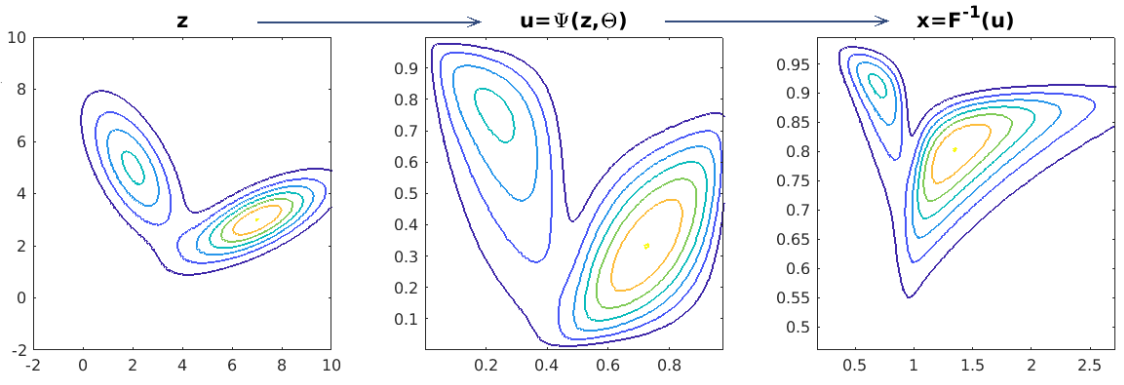
\includegraphics[width= 245pt]{figures/figure_gmcm_transformation}
\caption{Illustration of the transformations induced by a GMCM. The left panel shows the density contours of a 2-component GMM with parameters $\bs{\alpha} = \{0.45, \ 0.55\}$, $\bs{\mu} =\{[2 \ 5], [7 \ 3] \}$ and  $ \Sigma= \{[1.5 \  -1.3 ; -1.3 \quad 3 ],[3 \quad 1.2 ; 1.2 \quad 1] \}$. The middle panel shows the contours under the transformation by the marginal distribution functions [equation \eqref{eq:marginal_CDF}]. The right panel shows the transformation  by the quantile functions of $Lognormal(0,0.5)$ and $Beta(10,2)$ distributions along $x$ and $y$ dimensions, respectively [equation \eqref{eq:marginal_iCDF}]. Note that $\bs{x}\in \mathbb{R}^+\times [0,\ 1]$ owing to the Lognormal and Beta marginals.}

\label{fig:gmcm_transformation}
\end{figure}
\subsection{A numerical scheme to compute $\Psi^{-1}_r(\cdot)$ and its partial derivatives} 
Section \ref{subsec:MLE_GMCM} emphasized the need a method to compute $\Psi^{-1}_r(\cdot)$ that does better than the linear scaling of previous interpolation-based methods. Here, a computationally efficient alternative is proposed where the desired inversion is sought as the root of the expression $\bs{u}_r-\Psi_r(z_r)$, thus opening door to a rich set of algorithms. For instance, the well-known \emph{secant-method} enjoys quadratic convergence in most cases \citep{diez2003}, thereby needing far less number of function evaluations than the interpolation-based inversion. However, this only partly solves the problem, since the partial derivatives of $\Psi^{-1}_r(\cdot)$ are also needed with respect to $\Theta_r=\{\alpha_l,u_r^l,\sigma_r^l\}_{l=1}^m$. Appendix \ref{apd:gmm_quantile_derivatives} provides the derivation of the aforementioned partial derivatives. One may argue the need of explicit derivatives, when PPLs offer automatic-differentiation capabilities. 

\section{Identifiability of GMCM}\label{sec:identifiability_GMCM}
Another issue that plagues GMCM is that of parameter \emph{non-identifiability}. Identifiability is a key property that determines if it is possible to learn the true values of a generative model's parameters after observing infinite samples from it. Finite mixture models are known to suffer from the issue of parameter non-identifiability, since the likelihood is invariant under a permutation of component labels \citep[see][]{Stephens2000}. This is commonly known as \emph{label switching} problem. However, GMCM suffer from another form of parameter non-identifiability as proven in the theorem below.

  

\textbf{Theorem 1:} Let $U$ be a dataset generated by a $m$-component Gaussian Mixture Copula distribution with true parameters set $\Theta^* = \{\bs{\mu}^{l*}, \Sigma^{l*}, \alpha^{l*}\}_{l=1}^m$. Denote the log-likelihood of the observed data, with respect to the true model, as $\ell_\zeta(\Theta^*|U)$. Define another parameter set $\Theta= \{A\bs{\mu}^{l*}+\bs{b}, \ A^T\Sigma^{l*}A, \ \alpha^{l*}\}_{l=1}^m$, where $A$ is any diagonal positive definite matrix and $\bs{b}$ a real vector. Then, $\ell_\zeta(\Theta|U) = \ell_\zeta(\Theta^*|U)$.

 

\textbf{Proof}:  Let $\bs{z}\in \mathbb{R}^d$ is drawn from a $m$-component Gaussian mixture distribution with parameters $\Theta^* = \{\bs{\mu}^{l*}, \Sigma^{l*}, \alpha^{l*}\}_{l=1}^m$. Define strictly increasing transformations i.e. $\bs{w}_r = a_r \bs{z}_r+b_r$, with $a_r \in \mathbb{R}^+$ and $b_r \in \mathbb{R}$. Then $\bs{w}= [\bs{w}_1, \bs{w}_2,\ldots \bs{w}_d]$  has a Gaussian mixture distribution with parameters  $\Theta= \{A\bs{\mu}^{l*}+\bs{b}, \ A^T\Sigma^{l*}A, \ \alpha^{l*}\}_{l=1}^m$, where $A = \text{diag}([a_1, a_2, \cdots a_d])$ and $\textbf{b}=[b_1, b_2, \cdots b_d]$.

 

The vector $\bs{u}\in [0,1]^d$, such that $\bs{u}_r = \Psi_r(\bs{z}_r;\Theta^{*r}); r=1,2,\cdots, d $, has the joint density function (see definition 2 of GMC distribution) given by equation \eqref{eq:true_GMC_density}.

\begin{align}\label{eq:true_GMC_density}
\zeta(\bs{u};\Theta^*) & = \left( \frac{\psi\left(\bs{z};\Theta^*\right)}{\prod\limits_{r=1}^{d}\psi_r\left(z_r;\Theta^{r*} \right)} \right)
\end{align}

Likewise, the density function of $\bs{v}\in [0,1]^d$ such that $\bs{v}_r = \Psi_r(\bs{w}_r;\Theta^r); r=1,2,\cdots, d $ has the density function given by equation \eqref{eq:transformed_GMC_density}.

\begin{align}\label{eq:transformed_GMC_density}
\zeta(\bs{v};\Theta) & = \left( \frac{\psi\left(\bs{w};\Theta\right)}{\prod\limits_{r=1}^{d}\psi_r\left(\bs{w}_r;\Theta^r \right)} \right)
\end{align}

However, since cumulative distribution function values remain invariant under strictly increasing transformations, we have $\bs{u} \equiv \bs{v}$. This means $\bs{u}$ and $\bs{v}$ have the same generative distribution, or equivalently $\zeta(\textbf{u};\Theta^*) = \zeta(\textbf{u};\Theta)$. Therefore, the corresponding likelihood functions, defined on a dataset with $n$ samples $(U \in [0 , 1]^{d\times n})$, are equal for the two parameter configurations $\Theta^*$ and $\Theta$ i.e. $\ell_\zeta(\Theta|U) = \ell_\zeta(\Theta^*|U)$. This completes the proof. A practical repercussion of this result is that the true parameters of a GMC distribution can never be uniquely identified $-$even after addressing the label switching problem$-$ because the likelihood function has infinitely many maximizers. Readers can refer to \citet{White1982} for a detailed exposition on the subject of identifiability in parametric models. \citet{Bilgrau2016} noted this form of non-identifiability in GMCM, although did not prove it. They proposed an ad hoc solution that involved enforcing the first component to have zero mean and unit variance along each dimension. Nevertheless, as noted in their paper, the non-identifiability issue persisted under certain conditions. Here an alternative solution, formalized in theorem 2, is proposed that renders GMCM identifiable up to the permutation of component labels.

 

\textbf{Theorem 2:} Denote $\bs{g}\in \mathbb{R}^d$ and $\bs{h}\in \mathbb{R}^{+d}$ as real-valued vectors; the latter being positive. A $m$-component, $d$-dimensional Gaussian Mixture Copula distribution parametrized by $\Theta = \{\bs{\mu}^l, \Sigma^l, \alpha^l\}_{l=1}^m$ is identifiable, up to the permutation of component labels, if and only if the following two conditions are met for any $\bs{g}$ and $\bs{h}$.

\begin{align}
&\sum_{l=1}^m \alpha^l \ \bs{\mu}_r^l=\bs{g}_r \ ,\qquad \forall r \in \{1,2,\cdots,d\} \nonumber \\
&\sum_{l=1}^m \big[ \alpha^l \left(\Sigma_{rr}^l+(\bs{\mu}_r^l)^2\right)\big] -\bs{g}_r^2 =\bs{h}_r ,\qquad \forall r \in \{1,2,\cdots,d\}\nonumber
\end{align}

\textbf{Proof}: The proof is straightforward in the light that the LHS of the two equations above correspond to the mean and the variance of the marginals of a GMM, respectively. Affixing the vectors $\bs{g}$ and $\bs{h}$ to pre-specified values, therefore, prohibits the transformations that cause non-identifiability  (refer to proposition 2). Intuitively, by fixing the margins of the GMM (as we only seek the dependence structure it encodes), we eliminate different parameter configurations that encode the same dependence structure. Conversely, any parameter update that abides by the above two constraints, would result in non-increasing transformations, thus mitigating the non-identifiability noted in proposition 2. The choice of $\bs{g}$ and $\bs{h}$ is rather arbitrary. For convenience, the former can be set as $\mathbf{0}^d$ (vector of all zeros) and the latter $\mathbf{1}^d$ (vector of all ones).

\section{The EM algorithm for GMCM}\label{sec:EM}
The EM algorithm has garnered popularity for MLE in mixture models given that it 1) automatically satisfies the probabilistic constraints, 2) doesn't require explicit gradients, and 3) dispenses with the learning rate needed for other gradient-based approaches. The underpinning of EM is a two step process, the \emph{Expectation} (E)-step that finds a lower bound of the \emph{incomplete data} log-likelihood function (e.g., in Equation \eqref{eq:gmcm_logL}), and the \emph{Maximization} (M)-Step optimizes this lower bound (either partially or fully) to arrive at the next iterate. A repeated application of the E and M steps ensures monotonic increase of the data log-likelihood until local convergence is achieved. Readers may refer to \citet{Bilmes98agentle} and \citet{Salakhutdinov2002} for detailed treatments on the EM algorithm for GMMs. Although, the EM algorithm for GMCMs would follow the same general construct, the E and the M steps are considerably harder than those of GMM. The previous attempts at it \citep{Tewari2011, Bhattacharya2014} do not, systematically, derive and maximize the true lower bound of the incomplete data log-likelihood. Instead, certain assumptions are made that allow tweaking of the GMM's EM algorithm for learning GMCM's parameter. As a result, both of these algorithms need additional checks, at each iteration, to ensure monotonically increasing likelihood function. They are referred as pseudo-EM (PEM) algorithms for later benchmarking experiments. In summary, a provably correct EM algorithm has remained elusive for GMCM, and we close that gap here.
\subsection{E-Step} \label{subsec:EStep}
The ensuing derivation closely follows the exposition in \citet{Bilmes98agentle}, which presents EM algorithm for GMM in great details. Assuming access to $\bs{y}$, a $n$-dimensional vector of latent variables that co-occurs with the observed data $U$, the \emph{complete data} log-likelihood function can be written as,
\begin{equation}\label{eq:gmcm_complelte_logL}
\ell_{comp}(\Theta |U,\bs{y})= \sum\limits_{i=1}^{n} \log \left( \frac{\alpha^{\bs{y}_i}\phi \left(\invCDF{:i};\Theta^{\bs{y}_i} \right)}{\llDenom{i}} \right) .
\end{equation}
The latent variable $\bs{y}_i$ denotes the index of the Gaussian component from which the dependence of the $i^{th}$ data sample $U_{:i}$ is derived. The function $\phi(\cdot)$ is the multivariate Gaussian density,  $\Theta^{\bs{y}_i}$ and $\Theta^r$ represent the parameters associated with the $\bs{y}_i$ component and the dimension $r$, respectively. Also, $\invCDF{:i}$ and $Z_{ri}$ are used to denote $\Psi^{-1}\left(U_{:i}\right)$ and $ \Psi_r^{-1}(U_{ri})$, respectively. Note that the denominator does not depend on the latent variable $\bs{y}_i$, since the marginal densities, $\psi_r(\cdot)$ are not component specific. The E-step involves derivation of the expected value of the complete data log-likelihood (Equation \ref{eq:gmcm_complelte_logL}) with respect to the posterior distribution of the latent variables given the data and the current parameter estimates, say $\hat{\Theta}$. This posterior distribution in this case is $P(\bs{y}|U,\hat{\Theta}) = \prod\limits_{j=1}^{n}P\left(\bs{y}_j|U_{:j},\hat{\Theta} \right)$. Following some tedious but straightforward manipulations (cf. \ref{sec:Estep_derivation} for details) the expectation of complete data log-likelihood, $Q(\Theta,\hat{\Theta})$, can be written as,
\begin{align}\label{eq:GEM_objective}
Q(\Theta,\hat{\Theta}) =&  \sum\limits_{i=1}^n \sum\limits_{\bs{y}_i=1}^m  \left( \log (\alpha^{\bs{y}_i}) - \frac{\log(|\Sigma^{\bs{y}_i}|)}{2}\right) G_{i\bs{y}_i}  \nonumber \\ 
& -\sum\limits_{i=1}^n \sum\limits_{\bs{y}_i=1}^m  \left( \frac{\zbar{i}^T(\Sigma^{\bs{y}_i})^{-1}\zbar{i}}{2} \right) G_{i\bs{y}_i}  \nonumber \\
& -\sum\limits_{i=1}^n \sum\limits_{r=1}^{d} \log \left(\psi_r(Z_{ri};\Theta^r \right) ,
\end{align}
where $\zbar{i}=Z_{:i}-\mu^{\bs{y}_i}$ is the mean adjusted vector. It should be noted that, unlike the GMM, the E-step in GMCM does not completely remove the logarithm over sum of exponential terms (see in the third term of the Equation \ref{eq:GEM_objective}). Thus, the maximization of \eqref{eq:GEM_objective} does not yield closed-form updates for the model parameters $\Theta$ (as is the case with GMM); thereby necessitating a gradient-based M-step. Therefore, it can be argued that the EM algorithm does not enjoy the same benefits for GMCMs \textemdash as it does for GMMs\textemdash over the direct likelihood maximization. Nevertheless, the accurately derived E-step can still be maximized (or partially maximized) with a gradient-based M-step while guaranteeing monotonically increasing incomplete data log-likelihood function (unlike the PEM algorithms proposed in previous works).

\section{Experimental Results}\label{sec:Experimental}
This section provides empirical evidence to support the claims made in this paper using synthetic and real-world datasets. The experiments are carried out in Python.  The experiments aim to convey three key messages, 1) GMCM becomes identifiable in accord with the statement of theorem 1, 2) the proposed EM algorithm outperforms the previously published  PEM algorithms, and 3) density estimation via GMCM is comparable on  publicly available real-world datasets for the task of density estimation and compare GMCM's performance with a few other density estimators suited for data with complex non-Gaussian distributions. For other real-world applications, readers may refer to ~\cite{Bilgrau2012quantification,Wang2014,Yu2013GMCMWindPred,Bayestehtashk2015}, where GMCMs are used for tasks such as prediction, classification, anomaly detection, dependence characterization etc.

For the first experiment, a three-dimensional synthetic dataset is generated using the following procedure. An arbitrary $3$-component GMM is instantiated such that the conditions in theorem 1 are satisfied with $\bs{g}$ and $\bs{h}$ being vectors of all zeros and ones, respectively. One thousand random samples are generated from it. For each dimension, samples are transformed to obtain the univariate CDF values with respect to the marginal distribution induced by the multivariate GMM. This procedure results in a matrix $U \in [0 \ 1]^{3\times 1000}$, which serves as the training dataset to learn a GMC distribution using the GEM algorithm outlined in this paper. The emphasis here is on the ability to recover the \emph{true} model parameters of the aforementioned GMM. Figure \ref{fig:identifiability_exp} juxtaposes the result of the EM algorithm \textbf{with} (left panel) and \textbf{without} (right panel) the identifiability constraints. Starting from the same initial point (blue stars), the plots show the evolution of the iterates up to 400 iterations. The red squares and the yellow circles show the true model parameters and the parameters after 400 iterations, respectively. The divergence of iterates from the ground truth in quite apparent for the plots in the right panel. On the contrary, the iterates converge to the true parameter values (left panel) when the GEM algorithm enforces the identifiability constraints. Although the results are shown only for the mean parameters $\{\bs{\mu}^l \}_{l=1}^3$, the same holds true for other model parameters. Bear in mind that the identifiability constraints do not impose any restrictive assumption on the generative process of real-world datasets. They are merely making an ill-posed problem (with multiple equivalent solutions), well-posed (with a unique global solution) (see theorem 1). \\

\emph{Remark}: An important theoretical question that hasn't been probed in this paper is; how does the improved identifiability of GMCM impact the convergence of the GEM algorithm? Another interesting but unexplored aspect pertains to the parameter estimation in a Bayesian setting, where the non-identifiability of a model may cause performance issues in posterior approximations \citep[see][]{Neath1997}.

\begin{figure}[ht]
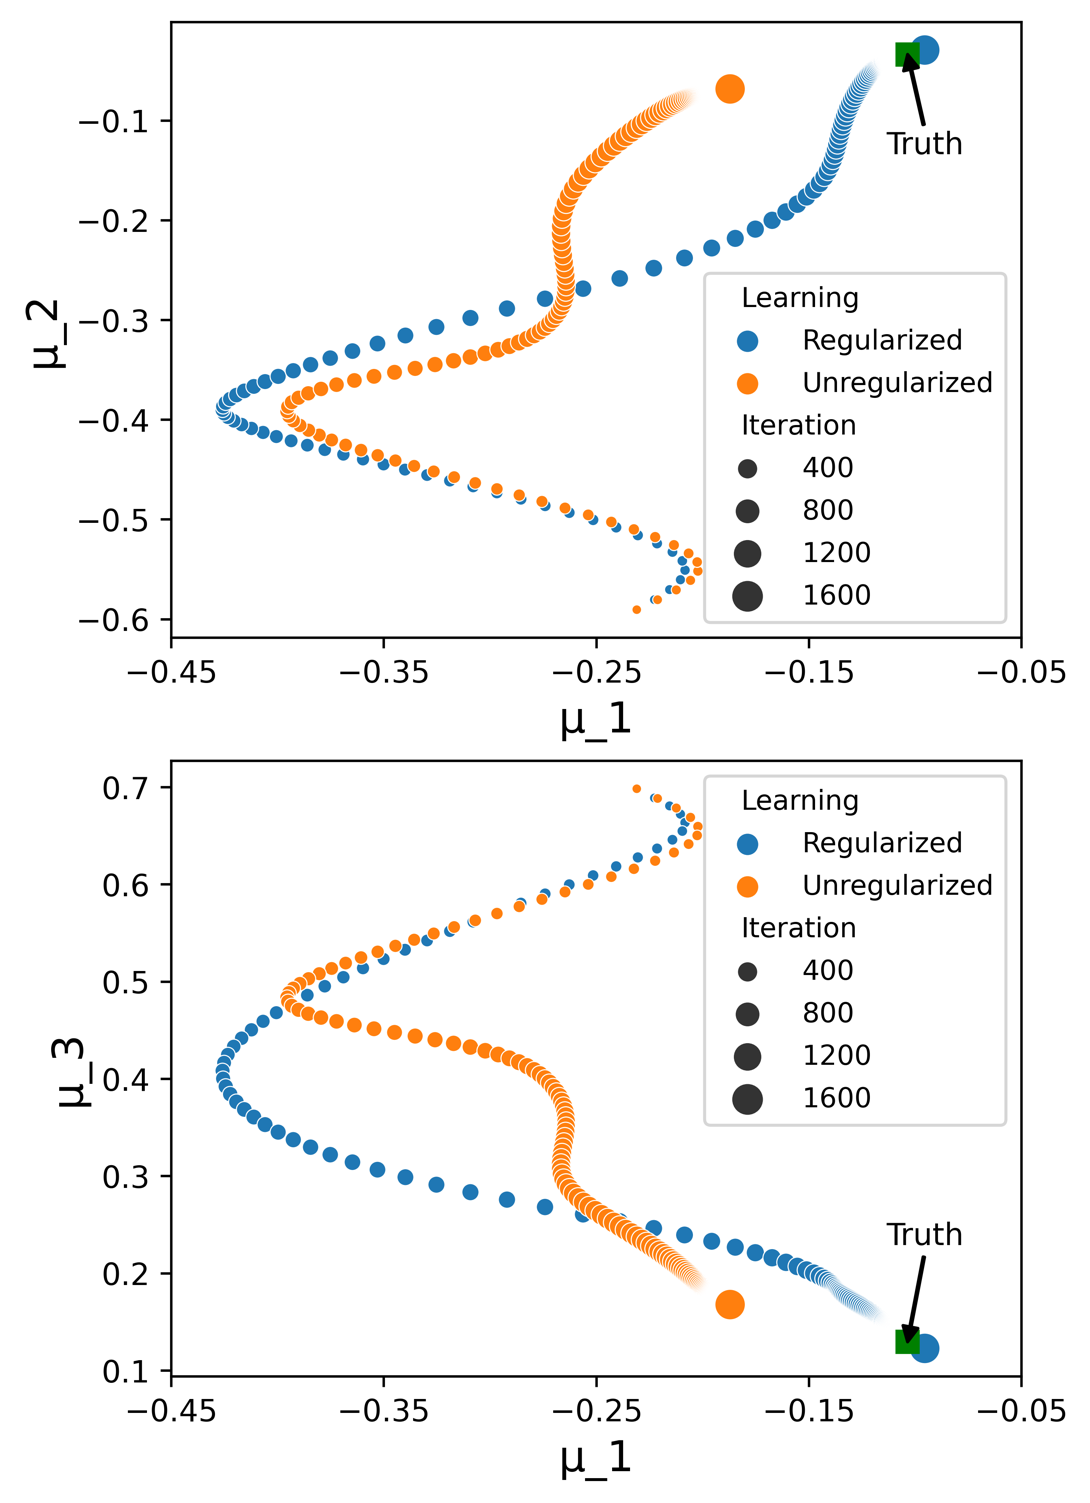
\includegraphics[width= 240pt,keepaspectratio]{figures/Identifiability_Experiment.png}
\caption{Manifestation of identifiability in GMC distribution shown empirically. Both plots show the evolution of the mean parameters ($\mu_i$), from a same initial point until convergence (2000 iterations), with and without regularization via identifiability constraints put forth in Theorem 1. The true values of the  parameters are shown by green squares.}
\label{fig:identifiability_exp}
\end{figure} 

The second experiments compares the performance of GEM algorithm with the two pseudo-EM algorithms published in \citet{Bhattacharya2014} and \citet{Tewari2011}, referred here as PEM$_1$ and PEM$_2$, respectively. The key performance indicator here is the log-likelihood value attained at the convergence of these algorithms. To ensure an exhaustive comparison, 100 datasets are generated by following the same procedure as in experiment 1. For each dataset, the GMC parameters are learned by the three algorithms with identical initialization. Figure \ref{fig:EM_algo_comp}(a) plots the log-likelihood vs. iteration, from the three algorithms, for one such dataset. GEM can be seen to converge to a higher log-likelihood value compared to PEM$_1$ and PEM$_2$. This observation is quite consistent over other datasets. Figure \ref{fig:EM_algo_comp}(b) summaries the results over all the datasets by showing the box-plots of the log-likelihood ratios, $\log\left( \frac{\mathcal{L}\left(\Theta^{GEM}|U\right)}{\mathcal{L}\left(\Theta^{PEM_1}|U\right)}\right)$ and $\log\left( \frac{\mathcal{L}\left(\Theta^{GEM}|U\right)}{\mathcal{L}\left(\Theta^{PEM_2}|U\right)}\right)$, of the converged models. A significantly positive median and the quantile values confirms the superior performance of GEM over PEM$_1$ and PEM$_2$.

\begin{figure}[ht]
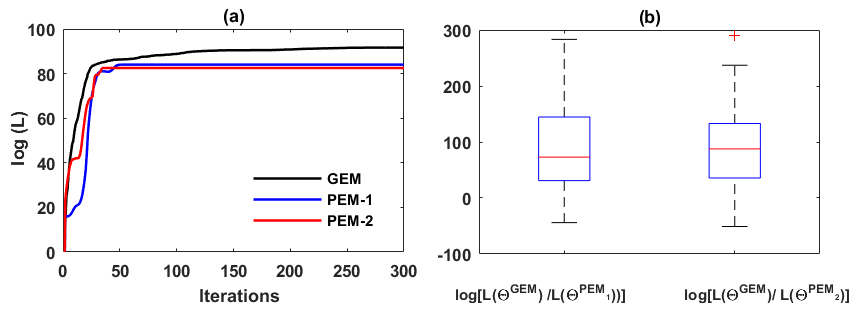
\includegraphics[width= 380pt,keepaspectratio=true]{figures/EM_algo_comparisons}
\caption{(a) log-likelihood vs. iteration for the three EM algorithms on a simulated dataset (b) Box-plots of converged log-likelihood ratios,  $\log\left( \frac{\mathcal{L}\left(\Theta^{GEM}|U\right)}{\mathcal{L}\left(\Theta^{PEM_1}|U\right)}\right)$ and $\log\left( \frac{\mathcal{L}\left(\Theta^{GEM}|U\right)}{\mathcal{L}\left(\Theta^{PEM_2}|U\right)}\right)$, by repeating this experiment on 100 such simulated datasets. The sub-optimal performance of pseudo-EM (PEM) algorithms is clearly evident.}
\label{fig:EM_algo_comp}
\end{figure}  

Finally, we evaluate GMCM's performance for the task of density estimation on real-world datasets of varying dimensions and sizes (see table \ref{tab:public_datasets} for details). In a recent work by \citet{Iwata2012}, \emph{infinite warped mixture model} (iWMM) is proposed for datasets with nonlinearly separable clusters with complex shapes. Belonging to the general class of \emph{Bayesian Non-Parametric} (BNP) models,  iWMM can be viewed as an extension to \emph{Gaussian process latent variable model}, GPLVM \citep{Lawrence2003} and \emph{infinite Gaussian mixture model}, iGMM \citep{Rasmussen1999}. \emph{Kernel Density Estimation} (KDE), another popular non-parametric method to model data with arbitrary complex distribution, is also included in the analysis for completeness. The implementation of all the methods, barring GMCM, is taken from \citep{Duvenaud2013}. The results, shown in table \ref{tab:DE_comparison}, are the average log-likelihood of test datasets in a 10-fold cross validation setting, similar to the one employed by \citet{Iwata2012}. A superior generative model should achieve higher likelihood value on test datasets. The GMCM usually achieved a higher test likelihood than the other competing methods. Additionally, the computational complexity of GMCM parameter estimation with respect to the number of data samples is $O(n)$ (refer to section \ref{subsec:complexity_analytic_grad}), as opposed to $O(n^3)$ for the BNP methods, rendering the former more amenable to large datasets with many samples.
 

\begin{table}
\centering
\caption{Summary of datasets used for comparing different density estimators. The datasets are procured from a public database, ODDS, that provides access to a large collection datasets to data science community for research purpose.}
\begin{tabular}{| c | c c c c c c c|}
\hline
& Iris & Glass  & Wine  & Vowel & Pima  & WBC  & Vertebral  \\
\hline
\textit{d} & 4                    & 9     & 13          & 12       & 8         & 30   & 6 \\
 \textit{n} & 150                & 214   & 129     & 528    & 768    & 378  & 240 \\
\hline
\end{tabular}
\label{tab:public_datasets}
\end{table} 

\section*{\refname}

% In the unusual situation where you want a paper to appear in the

% references without citing it in the main text, use \nocite

%\nocite{langley00}

\bibliography{citations}

\bibliographystyle{icml2022}

 

%%%%%%%%%%%%%%%%%%%%%%%%%%%%%%%%%%%%%%%%%%%%%%%%%%%%%%%%%%%%%%%%%%%%%%%%%%%%%%%

%%%%%%%%%%%%%%%%%%%%%%%%%%%%%%%%%%%%%%%%%%%%%%%%%%%%%%%%%%%%%%%%%%%%%%%%%%%%%%%

% APPENDIX

%%%%%%%%%%%%%%%%%%%%%%%%%%%%%%%%%%%%%%%%%%%%%%%%%%%%%%%%%%%%%%%%%%%%%%%%%%%%%%%

%%%%%%%%%%%%%%%%%%%%%%%%%%%%%%%%%%%%%%%%%%%%%%%%%%%%%%%%%%%%%%%%%%%%%%%%%%%%%%%

\newpage

\appendix

\onecolumn

\section{Appendix} 

\subsection{Glossary of frequently used symbols} \label{apd:symbol_glossary}
\begin{table}[h]
\caption{Symbols and descriptions}
\label{tab:symbol_glossary}
\begin{tabular}{ll}
\hline
\textbf{Symbol} & \textbf{Description} \\
\hline
$d$ & data dimensions \\
$m$ & number of components in the mixture model \\
$n$ & number of data samples \\
$\Theta = \{\bs{\mu}^l, \Sigma^l, \alpha^l\}_{l=1}^m$ & parameter of $m$-component, $d$-dimensional GMM \\
$\Theta^r= \{\bs{\mu}_r^l, \Sigma_{rr}^l, \alpha^l\}_{l=1}^m$ & parameters of marginal GMM along the $r^{th}$ dimension $(\Theta^r \subset \Theta)$ \\
$f_r $ & arbitrary univariate density function \\
$F_r, F_r^{-1}$ & the distribution and the quantile function corresponding to $f_r$ \\
$F$ & vector function defined as $F = [F_1, F_2,\cdots,F_d]$ \\
$\psi, \Psi$ & joint density and distribution function of GMM in $\mathbb{R}^d$ \\
$\psi_r , \Psi_r$ & density and distribution function of the of the GMM along the $r^{th}$ dimension \\
$\Psi_r^{-1}$ & quantile function corresponding to $\Psi_r$ \\
$\Psi^{-1}$ & vector function defined as $\Psi^{-1} = [\Psi_1^{-1}, \Psi_2^{-1},\cdots,\Psi_d^{-1}]$ \\
$\bs{x} \in \mathbb{R}^d$ & real valued vector whose distribution is sought \\
$\bs{u} \in [0,1]^d=F(\bs{x})$ &  vector of uniformly distributed random variables \\
$\bs{z} \in \mathbb{R}^d =\Psi^{-1}(\bs{u}) $ &  vector with quantile values of GMM marginals \\
$X \in \mathbb{R}^{d \times n}$ & matrix of $n$, $\bs{x}$ vectors arranged columnwise \\
$U \in [0,1]^{d \times n}$ & matrix of $n$, $\bs{u}$ vectors arranged columnwise \\
$Z \in \mathbb{R}^{d \times n}$ & matrix of $n$, $\bs{z}$ vectors arranged columnwise \\
$\bs{y}$ & $n$-dimensional vector such that $\bs{y}_i \in \{1,2,\cdots,m\}$ \\
$\bar{Z}_{:i} \in \mathbb{R}^d$ & mean adjusted vector i.e. $\bar{Z}_{:i} = Z_{:i} - \bs{\mu}^{\bs{y}_i}$ \\
$W $ & Cholesky factor of an inverse covariance matrix i.e. $W^TW=\Sigma^{-1}$ \\
\hline
\end{tabular}
\end{table}

\subsection{Derivation of E-Step}
Hence the expectation of the complete data log-likelihood can be written as

\begin{align} \label{eq:ll_comp_expectation}
Q(\Theta,\hat{\Theta})&=\sum\limits_{\bs{y}^1=1}^m \ldots \sum\limits_{\bs{y}^n=1}^m \left[ \left( \sum\limits_{i=1}^{n}H_{i\bs{y}_i}  \right) \prod\limits_{j=1}^{n}G_{j\bs{y}_j} \right] \text{  where,}
\end{align}

\begin{align}
H_{i\bs{y}_i} &= \log \left(\frac{\alpha^{\bs{y}_i}\phi(\invCDF{:i}; \Theta^{\bs{y}_i})}{\llDenom{i}} \right),\quad\text{and}\quad
G_{j\bs{y}_j} = P\left(\bs{y}_j|U_{:j},\hat{\Theta}\right) \nonumber
\end{align}

with $H$ and $G$ being matrices of dimensions $n\times m$. The $(j,l)^{th}$ element of the matrix $G$ denotes the posterior probability of the $l^{th}$ component given the $j^{th}$ sample and the current parameter estimate $\hat{\Theta}$, and is computed as

\begin{align}
G_{jl}=P\left(\bs{y}_j=l|U_{:j},\hat{\Theta}\right)=\frac{\alpha^l\phi\left(\Psi^{-1}(U_{:j}); \hat{\Theta}^l\right)}{\sum_{i=1}^m\alpha^i\phi\left(\Psi^{-1}(U_{:j}); \hat{\Theta}^i\right)}.
\end{align}

\subsection{Partial derivatives of $\Psi^{-1}_r(\cdot)$}\label{apd:gmm_quantile_derivatives}
Let's say that $z_r=\Psi_r^{-1}(u)$. Even though $\Psi^{-1}_r(\cdot)$ does not have a closed-form, its partial derivatives can be obtained analytically via its forward function $\Psi_r(\cdot)$, and by invoking Euler's chain rule, as shown in Equation \eqref{eq:TripleProduct}.
\begin{equation}\label{eq:TripleProduct}
\frac{dz_r}{d\theta}=- \frac{\left(\frac{d\Psi_r(z_r)}{d\theta}\right)_z}{\left(\frac{d\Psi_r(z_r)}{dz_r}\right)_\theta}
\end{equation}
The expression in the denominator is identical for all the partial derivatives and is simply the density functionof the univariate GMM, i.e 
\begin{equation}\label{eq:Gamma_dz}
\der{z_r}{\Psi_r(z_r)}=\psi_r(z_r).
\end{equation}
The partial derivatives of the numerator can be derived, as follows, by applying of matrix calculus identities.
\\
\\
\text{Derivative of $z_r$ w.r.t to $\alpha_k$}
\begin{equation}
\der{\alpha_k}{\Psi_r(z_r)}=\frac{1}{2}\left[1+ \erf \left( \frac{z_r-\mu_{k,r}}{\sqrt{2\Sigma_{r,k}}}\right) \right]
\end{equation}
\\
\text{Derivative of $z_r$ w.r.t to $\mu_k$}
\begin{equation}
\der{\mu_k}{\Psi_r(z_r)}= -\frac{\alpha_k}{\sqrt{2\pi\Sigma_{r,k}}}\exp\left( - \frac{(z_r-\mu_{k,r})^2}{2\Sigma_{r,k}}	 \right)
\end{equation}
\\
\text{Derivative of $z_r$ w.r.t to $\Sigma_k$}
\begin{equation}
\der{\Sigma_k}{\Psi_r(z_r)}= -\sum\limits_{l=1}^{m}\frac{\alpha_l}{\sqrt{2\pi\Sigma_{r,l}}}\exp\left( - \frac{(z_r-\mu_{r,l})^2}{2\Sigma_{r,l}} \right) \times \frac{(z_r-\mu_{r,l})}{2\Sigma_{r,l}} \times \der{\Sigma_k}{\Sigma_{r,l}}
\end{equation}


\end{document}